%!TEX root = ../dissertation.tex

\chapter{Background}
\label{chapter:background}

%\section{The Internet of Things}

\section{Low Power Wide Area Networks}

The number of \gls{IoT} devices is expected to grow significantly in the years to come. The year 2017 will be remembered as the year in which the number of connected devices surpassed the world population \footnote{https://www.statista.com/statistics/764026/number-of-iot-devices-in-use-worldwide/}.
In many applications, such as smart cities, environmental monitoring and smart agriculture, these devices are densely deployed and powered by traditional AA batteries. For these reasons, they must be able to operate under strict power constraints using simple and cheap hardware components. Transmitting data over a wireless medium is a very costly operation in terms of power, due to many unpredictable environmental factors such as heat, humidity, wind and buildings and due to the inherent complexity of traditional wireless technologies.
Protocols like \gls{BLE} and ZigBee try to address the power limitation problem when short-range communication is needed, but for a vast number of IoT applications, where a high number of devices are deployed over large areas (e.g. a city), these short range solutions are suboptimal and expensive due to the complex and dense network infrastructure that needs to be installed. Cellular networks cover large areas, but are not power efficient. Moreover 2G, 3G and LTE connectivities are typically available in urban areas, but not always in suburban or rural areas. To address the aforementioned problems, a new range of protocols and technologies are being developed with the explicit purpose of enabling the operation of \glspl{LPWAN}. As the name suggests, \glspl{LPWAN} have the primary objective of providing low-power and low-cost connectivity over large geographical areas. The applications are multiple and diverse: smart cities, smart grids, smart metering, logistics, industrial monitoring, smart agriculture, etc.
Recently, all the principal \glspl{SDO} such as the \gls{IETF}, the \gls{IEEE}, the \gls{3GPP} and the \gls{ETSI} are intensifying their efforts in the standardization of \gls{LPWAN} protocols. Moreover, numerous consortiums and alliances works to promote specific \gls{LPWAN} technologies. Examples of such alliances are the LoRa Alliance promoting the LoRaWAN protocol, the Dash7 Alliance promoting the Dash7 Alliance protocol and the Wightless-SIG promoting the Weightless protocol. Even if the existing \gls{LPWAN} protocols and solutions are extremely diverse and address different niches in the same application segment, most of them use similar solutions to solve the same range of problems. A quick summary is given below:

\begin{itemize}
\item \textbf{Use of sub-GHz bands:} the vast majority of \gls{LPWAN} protocols take advantage of the good qualities of sub-GHz bands in terms of attenuation, multipath fading and obstacle penetration. Moreover, sub-GHz bands are currently less congested than the overly used 2.4 GHz band. Most \gls{LPWAN} technologies (e.g. LoRa and Sigfox) use unlicensed \gls{ISM} bands, while cellular operators are trying to exploit already owned licensed frequency bands. The use of unlicensed \gls{ISM} bands reduces the operational costs of running the network, but with the drawback of having to compel with the rules mandated by legislative authorities for the usage of these bands. As an example, in Europe, the 868.0-868.6 MHz band is subject to a 1\% duty cycle limitation \cite{missing}, meaning that, in a day, a single device can transmit for at most 14.4 minutes.

\item \textbf{Use of \gls{NB} or \gls{SS} modulations:}\gls{NB} modulations have the advantage of reducing the adverse effects of noise on the transmitted signals. Using these techniques, receivers can successfully recover severely attenuated signals and achieve a sensitivity level of even -130 dBm \cite{missing}. On the other side, the small bandwidth only allows low data rates in the order of few kbps or even a few hundred of bps if an \gls{UNB} modulation is used. In this case the bandwidth can be as low as 100 Hz. Some protocols, such as LoRa, use variations of \gls{SS} techniques to spread the narrowband signal over a wider bandwidth. The resulting signal has noise-like characteristics that makes it more resistant to jamming and eavesdropping and more resilient to interference. To overcome the less efficient use of bandwidth, \gls{SS} is typically used in conjunction with orthogonal codes. This allows multiple overlapping signals that are spread using different codes to be successfully recovered at the receiver.

\item \textbf{Low power operation:} in a \gls{LPWAN}, end devices are typically battery-powered and might need to operate using the same battery for many years. To reduce power consumption, \gls{LPWAN} networks are organized in a simple and efficient star topology or a star-of-stars topology, where all the devices are directly connect to one or multiple gateways or base stations. Multi-hop protocols are typically not used since some network nodes, called hot-spots, might experience more traffic than the others. Moreover, hot-spots have to listen periodically for new messages coming from the other nodes thus reducing their overall battery lifetime. Duty-cycling the devices, i.e. alternating ON-OFF communication periods, is another frequently used technique to reduce the power consumption.
For example, an uplink transmission can start only when new data is ready and a downlink reception can start only at a predefined scheduled time, usually following an uplink transmission. Simple random access ALOHA-like MAC protocols, requiring simple and cheap hardware and no synchronization, are typically used. Finally, to save on computational power, some complex operations, like detecting duplicated packets, are offloaded to the backend network.

\item \textbf{Low cost deployment:} installing, maintaining and operating an \gls{LPWAN} network must be as cheap as possible. \glspl{LPWAN} can achieve a chip cost as low as 1-2 \$ with an annual operation cost of 1\$. This can be achieved by resorting to simple and sometimes inaccurate hardware components. The network backbone usually requires only few base stations to cover areas of tens of kilometres, thus additionally reducing the deployment cost of the network. Finally, most \gls{LPWAN} solutions use unlicensed \gls{ISM} bands thus avoiding wasting money for the acquisition of licenses.

\item \textbf{Scalability:} support of a large number of devices is usually achieved by diversifying as much as possible in time, space and channels. Since devices use simple hardware, this diversification is usually implemented in the backend by using multi-channel multi-antenna base stations to parallelise the reception of signals. Some protocols also implement mechanisms to dynamically adapt the data rate and to select the best channel, but given the strong link asymmetry of most \gls{LPWAN} solutions, this mechanism, highly reliant on downlink information transmitted by the base station, is quite limited.

\end{itemize}

%\subsection{LPWAN Technologies}

\section{LoRa}

LoRa is a proprietary modulation technique based on \gls{CSS} originally developed by Cycleo and then acquired by Semtech in 2012. As many other \gls{LPWAN} technologies, LoRa uses the unlicensed sub-GHz bands (868 MHz in Europe, 915 MHz in North America, 433 MHz in Asia), therefore taking advantage of the good propagation properties of the spectrum. Since the LoRa modulation is proprietary, no official comprehensive description of the modulation exists as of today, but many attempts to reverse engineer the protocol have been made. The description of the LoRa physical layer given in the present work is based on \cite{undefined}.

\subsection{LoRa Modulation}

\begin{figure}[h]
    \centering
    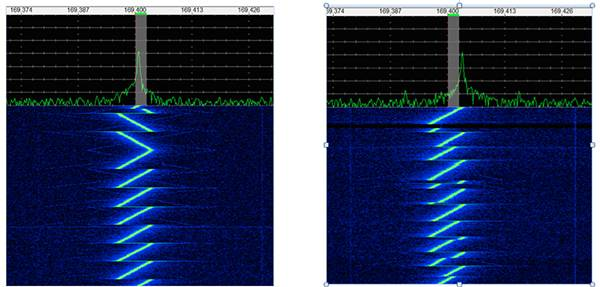
\includegraphics[width=0.9\textwidth]{images/lora-chirps.jpg}
    \caption{Visualisation of LoRa chirps \ref{undefined}}
    \label{fig:lora-chirps}
\end{figure}

The LoRa modulation is a variation of the \gls{CSS} modulation technique, which is in turn a subcategory of \gls{DSSS}. In \gls{DSSS} data is spread over a wider bandwidth by multiplying the transmitted symbol by a \gls{PN} sequence called chip sequence. The \gls{PN} sequence is generated with a frequency higher than the symbol generation frequency. The result is a signal with a very low \gls{SNR} that makes the it practically unrecognisable from background noise and very resilient to other \gls{RF} noise sources. The \gls{PN} sequence, known also by the receiver, is used to de-spread the signal and recover the original data. These properties make \gls{DSSS} an ideal solution for \glspl{LPWAN}. Unfortunately, \gls{DSSS} requires a highly accurate and expensive clock source to synchronize the \gls{PN} sequence at the transmitter and at the receiver. This makes traditional \gls{DSSS} not particularly suited for low-cost end devices such as the ones deployed in a \gls{LPWAN}.
\gls{CSS} is a variation of \gls{DSSS} initially used for radar systems and for a long time ignored in communication systems, but recently revalued due to its robustness to a wide range of channel degradation mechanisms such as multipath fading, signal fading, Doppler shift and jamming interferers.
In \gls{CSS}, the chip sequences are substituted by chirps, i.e. signals of continuously increasing or decreasing frequency inside a defined frequency range. An increasing frequency chirp is called up-chirp, while a decreasing frequency chirp is called down-chirp. To simplify transmitter and receiver's hardware, up-chirps and down-chirps are linear in frequency as is the case for LoRa.
In LoRa, a symbol is first chipped at a higher frequency that depends on the \gls{SF} and then modulated into a chirp. The chirp is characterized by the \gls{SF}, a minimum frequency $f_{min}$ and a maximum frequency $f_{max}$. An initial frequency $f_0$ is assigned to the symbol. The chirp sweeps the frequencies from $f_0$ to $f_{max}$, wrapping around from $f_{max}$ to $f_0$ when hitting the end of the available bandwidth $B = f_{max} - f_{min}$. The period of the chirp is determined by the equation \ref{eq:chirp_period}. The modulation data rate can then be computed as shown in equation \ref{eq:lora_dr}.

\begin{equation}
\label{eq:chirp_period}
T_C = \frac{2^{SF}}{B} secs
\end{equation}

\begin{equation}
\label{eq:lora_dr}
R_b = SF*\frac{1}{T_C} bits/s
\end{equation}

From equations \ref{eq:chirp_period} and \ref{eq:lora_dr}, it is possible to observe that a bigger \gls{SF} corresponds to a longer chirp period and consequently a lower data rate. On the other side a higher \gls{SF} makes the signal more resilient to noise and other \gls{RF} interferers, thus allowing for a lower receiver sensitivity and therefore the possibility of successfully recovering the signal from higher distances. This robustness is counterbalanced by a higher probability of collision, since the signal takes more time to be transmitted. In LoRa the \gls{SF} can vary between 7 and 12. If the coding rate is not considered, the typical LoRa data rates are presented in Table \ref{tab:lora_dr}.

\begin{table}[]
\centering

\begin{tabular}{|c|c|c|}
\hline
\textbf{SF} & \textbf{Bandwidth} & \textbf{Bitrate} \\ \hline
 12 & 125 kHz & 366 bps  \\ \hline
 11 & 125 kHz & 671 bps \\ \hline
 10 & 125 kHz & 1220 bps \\ \hline
  9 & 125 kHz & 2197 bps \\ \hline
  8 & 125 kHz & 3906 bps \\ \hline 
  7 & 125 kHz & 6835 bps \\ \hline 
\end{tabular}
\caption{LoRa Data Rates}
\label{tab:lora_dr}

\end{table}

\subsection{LoRa Physical Layer Packet}

Through a process of reverse engineering explained in \ref{undefined}, the authors were able to infer the structure of the LoRa physical layer packet. The packet has three fields:

\begin{itemize}

\item \textbf{Preamble:} used for the synchronization between the receiver and the transmitter. It's composed of a variable sequence of up-chirps having the same duration;

\item \textbf{\gls{SFD}:} indicates the beginning of a frame. It's composed by 2 down-chirps;

\item \textbf{Header and Data:} up-chirps of varying length. The data is extracted from the instantaneous frequency transitions of the chirps.

\end{itemize}

Some additional techniques are used to increase the robustness of the LoRa modulation:

\begin{itemize}

\item \textbf{Gray Indexing:} before being transmitted, the symbols are Gray indexed. Gray indexing is a way of encoding digits such that two consecutive digits have a change only in one bit position. This allows for more error tolerance. In the actual implementation, the symbols are read as gray-coded and de-grayed before transmission. Therefore the decoder needs to gray-code the symbols to recover the original symbols;

\item \textbf{Data whitening:} this process induces randomness in the sequence of bits in order to reduce long sequences of repeating bits. This allows a better clock recovery by the receiver. The whitening is done by XORing the symbols with a pseudorandom sequence that is known by both the transmitter and the receiver;
    
\item \textbf{Interleaving:} the initial ordered sequence of bits is scrambled using a scrambling sequence. The receiver uses the inverse operation to reconstruct the original bit sequence. This technique is used in conjunction with \gls{FEC} to spread multiple consecutive errors over the whole frame. LoRa uses a variation of a diagonal interleaver;

\item \textbf{\gls{FEC}:} enables bits damaged during the transmission to be recovered at the receiver by introducing some redundancy in the transmitted data. LoRa implements a Hamming \gls{FEC} that substitutes a 4-bit word with a codeword with length in the range [5-8] bits. A longer codeword provides additional protection at the cost of additional bits. When an Hamming (5,4) or (6,4) is used, only error detection is available. A Hamming (7,4) can correct a single bit error, while a Hamming (8,4) can correct a two bit error.

\end{itemize}

To improve reliability, code diversity is also exploited. Different spreading factors use semi-orthogonal codes, thus enabling the recovery of two signals overlapping in time and frequency if they have different \glspl{SF}. This feature enables the network to achieve a higher overall throughput, thanks to the fact that colliding packets with different \glspl{SF} can still be correctly demodulated.

\section{LoRaWAN}

The LoRaWAN standard \cite{undefined}, promoted by the LoRa Alliance, defines the network architecture and the MAC layer of an \gls{LPWAN} network that use the LoRa modulation. The complete LoRaWAN stack is shown in Figure \ref{undefined}. A brief overview of the main LoRaWAN characteristics and features is given in the following sections.

\subsection{Architecture and Topology}

\begin{figure}[h]
    \centering
    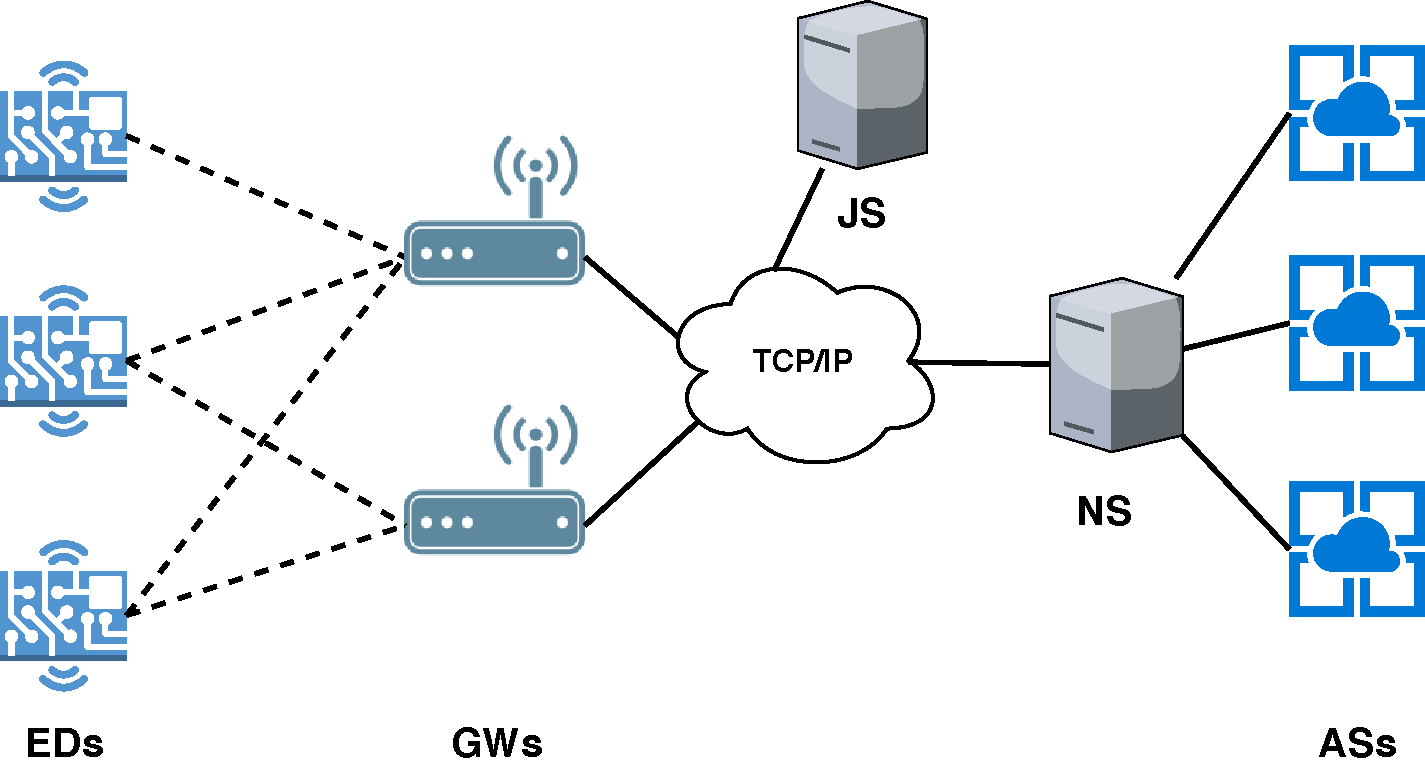
\includegraphics[width=0.95\textwidth]{images/lora-topology.pdf}
    \caption{Topology of a LoRaWAN network}
    \label{fig:lorawan-architecture}
\end{figure}

The overall architecture of LoRaWAN is shown in the picture \ref{fig:lorawan-architecture}.
LoRaWAN implements a star-of-stars topology interconnecting five different network elements:

\begin{itemize}
	\item \textbf{\glspl{ED}:} they are typically low-powered devices with sensing capabilities. \glspl{ED} transmit or receive data using the LoRa radio channel. They can establish communication only with LoRa gateways.
Once an \gls{ED} is registered in the network, uplink messages can be received by multiple gateways at once;

	\item \textbf{\glspl{GW}:} one or multiple gateways are responsible for collecting and aggregating the data coming from the \glspl{ED}. Gateways are responsible for demodulating the LoRa uplink transmissions and relaying the uplink messages to a network server using a traditional IP-based backhaul network. Upon request, \glspl{GW} can also send downlink messages to end nodes;
	
	\item \textbf{\gls{NS}:} collects the packets coming from the \glspl{GW} and routes them to the appropriate \gls{AS}. The \gls{NS} is also responsible of sending/receiving MAC commands and discard duplicated packets;
	
    \item \textbf{Application Servers (ASs)}: implement the application specific logic. An \gls{AS} aggregates, analyses and/or stores data and present it to the end users in a meaningful way. End users only interact with the services offered by an \gls{AS};
    
    \item \textbf{\gls{JS}:} manages \glspl{ED} activation. It derives and stores the keys used by the network for encrypting the communications.
        
\end{itemize}

\subsection{\glspl{ED} Operation Modes}

LoRaWAN defines three classes of \glspl{ED} with different characteristics and functionalities:

\begin{itemize}
 \item \textbf{Class A \glspl{ED}:} class A is the default operation mode of a LoRaWAN device. Class A \glspl{ED} open two short downlink receive windows immediately after an uplink transmission, therefore making this mode of operation best suited for \glspl{ED} that need a feedback from the network only after a successful transmission. The first receive window (RX1) is opened immediately after the uplink transmission. During RX1, the downlink frequency and data rate are set according to the same set of parameters used in uplink. In the second receive window (RX2), the downlink frequency and data rate are fixed and can be configured using specific MAC commands. Both RX1 and RX2 must stay open at least for the time needed for a \gls{GW} to detect the downlink preamble and are only closed when the eventual downlink transmission is completed. Thanks to the limited downlink time, Class A \glspl{ED} are the most power-efficient devices in a LoRaWAN network;
 
\item \textbf{Class B \glspl{ED}:} this class of devices retains all the functionalities of class A \glspl{ED}, but  additionally, class B \glspl{ED} can open additional receive windows at specific time instants agreed with the \glspl{GW}. \glspl{GW} must periodically send a beacon that specifies the exact time at which the additional receive windows must be opened. This feature allows for a more flexible use of the downlink channel, therefore representing a good compromise in terms of power consumption and chances of sending downlink messages;

\item \textbf{Class C \glspl{ED}:} \glspl{ED} operating in this mode keep the receiving windows continuously open, except when the ED is transmitting a message in uplink. Class C operation mode is the least power-efficient class and should be used only in \glspl{ED} with relaxed power constraints that benefit from low latency downlink messages.

\end{itemize}

All the \glspl{ED} must implement Class A operation mode and may optionally implement one or all of the other available classes. An \gls{ED} can switch to Class B or Class C operation modes by using specific MAC commands only after having successfully joined the LoRaWAN network. 

\subsection{MAC Frames and Commands}

\begin{figure}[h]
    \centering
    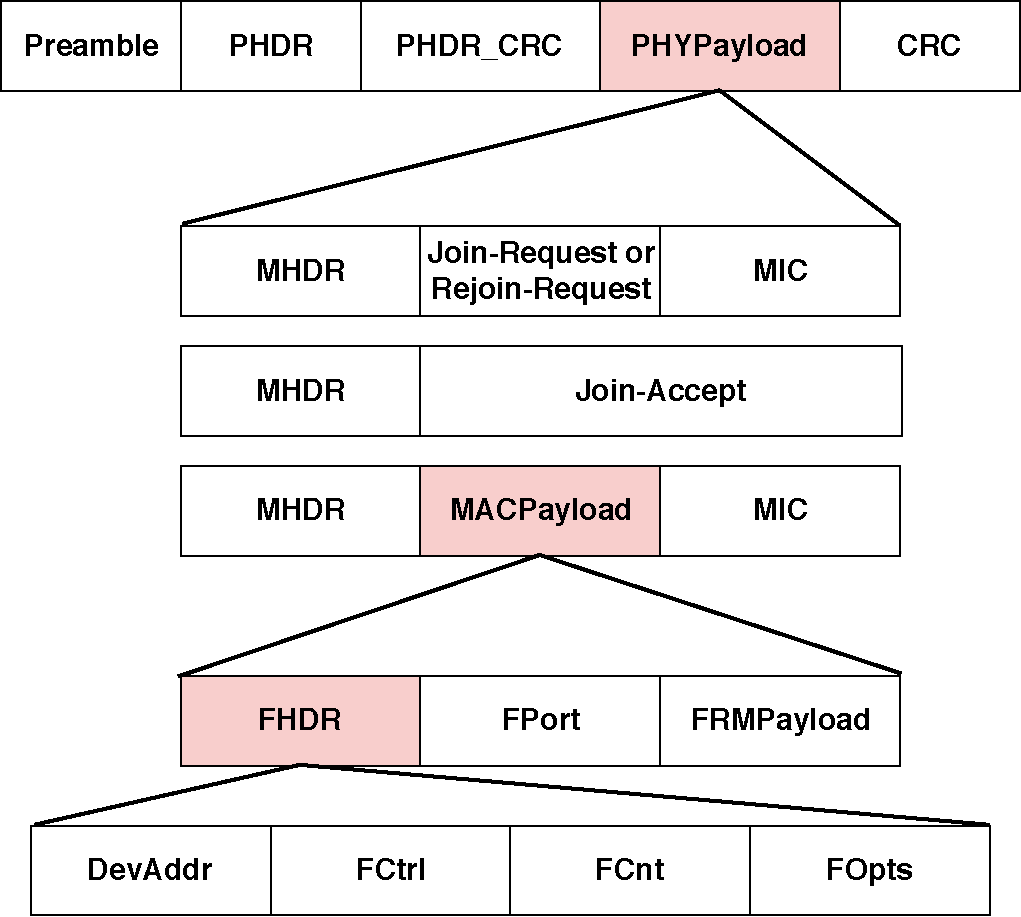
\includegraphics[width=0.9\textwidth]{images/mac-commands.pdf}
    \caption{MAC frames structure}
    \label{fig:lorawan-mac}
\end{figure}

The structure of LoRaWAN MAC frames is shown in Figure \ref{fig:lorawan-mac}.
MAC frames are encapsulated in the physical layer packet payload and are formed by a \gls{MHDR}, a MAC payload (MACPayload) and a \gls{MIC}, that is used to verify the integrity of the PHY payload. 
The \gls{MHDR} contains, among other fields, a 3-bit MType field that specifies the message type. The available types are listed in Table \ref{tab:mtypes}.

\begin{table}[]
\centering

\begin{tabular}{|c|c|}
\hline
\textbf{MType} \& \textbf{Description}\\ \hline
 000 & Join-Request  \\ \hline
 001 & Join-Accept \\ \hline
 010 & Unconfirmed Data Up  \\ \hline
 011 & Unconfirmed Data Down  \\ \hline
 100 & Confirmed Data Up \\ \hline 
 101 & Confirmed Data Down \\ \hline
 110 & Rejoin-Request \\ \hline  
 111 & Proprietary \\ \hline 
\end{tabular}
\caption{MAC message types (MTypes)}
\label{tab:mtypes}

\end{table}

Data messages are used for transmitting MAC commands and/or application data. A distinction is made between data messages that require an acknowledgement from the receiving device (an \gls{ED} or a \gls{GW}) and data messages that do not require an explicit acknowledgement. Join-request, Join-Accept and Rejoin-request messages are used for \gls{OTA} activation as described in section \ref{sec:activation}.  
The MACPayload field is additionally divided in \gls{FHDR}, \gls{FPort} and Frame Payload (FRMPayload). The \gls{FHDR} contains a 4-byte Device Address (DevAddr), a 1-byte Frame Control (FCtrl) to request the \gls{ADR} or an acknowledgement, a 2-byte Frame Counter (FCnt) and an optional Frame Options (FOpts) field containing up to 15 bytes of MAC commands. The mandatory 1-byte \gls{FPort} field is used to specify the port used by the application. This field is used by the \gls{NS} to route the message to the correct application in the \gls{AS}.
Other than data, LoRaWAN MAC frames can carry one or more MAC commands.  
MAC commands are simple commands exchanged exclusively between the \gls{NS} and the \glspl{ED}. MAC commands can be piggybacked to a data message using the FOpts field or they can be carried in the FRMPayload by specifying a FPort value of 0. Each command is defined by a 1-byte \gls{CID} followed by zero or more command specific octets.
MAC commands can be used to:

\begin{itemize}
 
    \item Check the line connectivity;
    \item Limit the duty cycle of an \gls{ED};
    \item Set the receive parameters of the second receive window;
    \item Request status info to \glspl{ED};
    \item Set the delay between a transmission and the opening of the first receive window;
    \item Change \gls{ADR} parameters;
    \item Request current time and date to the network.

\end{itemize}

\subsection{Adaptive Data Rate}

LoRaWAN specifies an \gls{ADR} mechanism that is used to optimize the data rate, transmission power and spectrum usage of \glspl{ED} according to the quality of the link as measured by different metrics. When \gls{ADR} is active, the \gls{SF} of the modulation is adjusted in order to match the quality of the channel: it is increased when the \gls{SNR} is low in order to increase the receiver sensitivity and decreased when the \gls{SNR} is well above the threshold in order to minimize the power consumption and the time-on-air of the messages. An \gls{ADR} request is always started by an \gls{ED} by setting the \gls{ADR} bit in the FCtrl field. This bit signals to the \gls{NS} that the node is willing to accept \gls{ADR} parameters variations based on the observations collected by the \gls{NS}. It's worth noting that the specification doesn't specify an algorithm to be used for \gls{ADR}, thus leaving the implementation details to the manufacturer of the network equipment or the network operator. The \gls{ADR} should only be used by static nodes or by "smart" mobile nodes that are able to detect when they are parked for an extended period of time.

\subsection{Activation of \glspl{ED}}

A LoRaWAN network implementation is by default protected by some security mechanisms that guarantee data integrity and confidentiality and prevent replay attacks. These three requirements are guaranteed respectively by \glspl{MIC}, 128 bits \gls{AES} encryption and nonces. All security features require the presence of a set of session keys, that must be derived during the \gls{ED} mandatory join procedure.
Each \gls{ED} must join the network using either \gls{OTA} activation or \gls{ABP}. The only difference between the two procedures is in the way in which the session keys are derived: in \gls{OTA} activation, keys are generated on-demand, while in \gls{ABP} keys are manually loaded. Only the most interesting \gls{OTA} activation is discussed in this section. \\

\subsubsection{OTA Activation}

Before starting the join procedure, each \gls{ED} is provided with four pieces of information that must be stored securely in the device:

\begin{itemize}
	\item \textbf{Join EUI:} a 64 bit global identifier of the \gls{JS} responsible for the join procedure;
	\item \textbf{Device EUI (DevEUI):} a 64 bit global identifier of the \gls{ED}. The DevEUI is typically written also on a label on the back of the \gls{ED};
	\item \textbf{Network Key (NwkKey):} an AES-128 root key, assigned when the \gls{ED} is manufactured, used to derive the Forwarding Network Session Integrity Key (FNwkSIntKey), the Serving Network Session Integrity Key (SNwkSIntKey) and the Network Session Encryption Key (NwkSEncKey);
	\item \textbf{Application Key (AppKey):} an AES-128 root key, assigned when the \gls{ED} is manufactured, used to derive the Application Session Key (AppSKey).
\end{itemize}

The join procedure is always started by an \gls{ED} by sending a Join-Request message to the \gls{JS} containing the Join EUI, the DevEUI and a Device Nonce (DevNonce). The DevNonce is used to avoid the occurrence of replay attacks. The \gls{ED} must store the last used DevNonce value and increment it at each subsequent Join-Request. The last value of the nonce is also permanently stored in the \gls{NS} and every time a message is received, the DevNonce is compared with the stored value. If the received nonce is lower than the value stored in the \gls{NS}, the message is discarded. If the \gls{JS} accept the \gls{ED} registration, a Join-Accept message is returned in downlink. The message contains the join nonce, the Network id (NetID), the 32-bit Device Address (DevAddr) and a set of network configuration parameters. The join nonce is also in this case a progressive number, but it is used to derive the session keys. After the completion of the join procedure, the following session keys are established:

\begin{itemize}

\item \textbf{FNwkSIntKey:} used by the \gls{ED} to compute the \gls{MIC} of all uplink messages;
\item \textbf{SNwkSIntKey:} used by the \gls{ED} to verify the \gls{MIC} of all downlink messages;
\item \textbf{NwkSEncKey:} used by the \gls{ED} and the \gls{NS} to encrypt/decrypt uplink and downlink MAC commands;
\item \textbf{AppSKey:} used by the \gls{ED} and the \gls{AS} to encrypt end-to-end the payload field of application-specific data messages. It's worth noting that even if confidentiality is guaranteed end-to-end, the integrity of messages is only guaranteed hop-by-hop, thus potentially allowing a malicious \gls{NS} to tamper with the data;

\end{itemize}


%\section{Other LPWAN protocols (?)}
%
%A section describing other LPWAN protocols. Irrelevant?
%
%\section{The WiFi Protocol (?)}
%
%A section describing the WiFi protocol. Even if it's used in the scenario, it's not the main focus. Irrelevant?
%
%\section{MANET routing algorithms (?)}
%
%A section describing routing algorithm for MANETs. Maybe move to implementation section to describe the routing algorithms available in ns-3 and the reason for the chosen algorithm.

\section{Ad hoc wireless networks}

\section{Unmanned Aerial Vehicles}

\gls{UAV} is a general term used to identify all aircraft that are able to fly without the presence of an on-board human pilot. Depending on the level of achieved autonomy, two additional categories of \glspl{UAV} with a lower degree of autonomy can be defined: \glspl{RPV} and drones. As the name suggests, \glspl{RPV} are not fully autonomous and need a complete or partial control of a remote pilot using some sort of remote control system (a joystick for example). Despite being used as a synonym of \gls{UAV}, drone is a term that should be more appropriately used to indicate "dumb" \glspl{UAV} only capable of fairly limited actions and with a just as limited set of functionalities (e.g. target drones). Since the use of drone as a synonym of \gls{UAV} is very common in both the academic literature and in the everyday language, in the rest of the present work the two terms are used interchangeably. 

\subsection{\glspl{UAV} classification}

\begin{figure}
\centering
\begin{subfigure}{.5\textwidth}
  \centering
  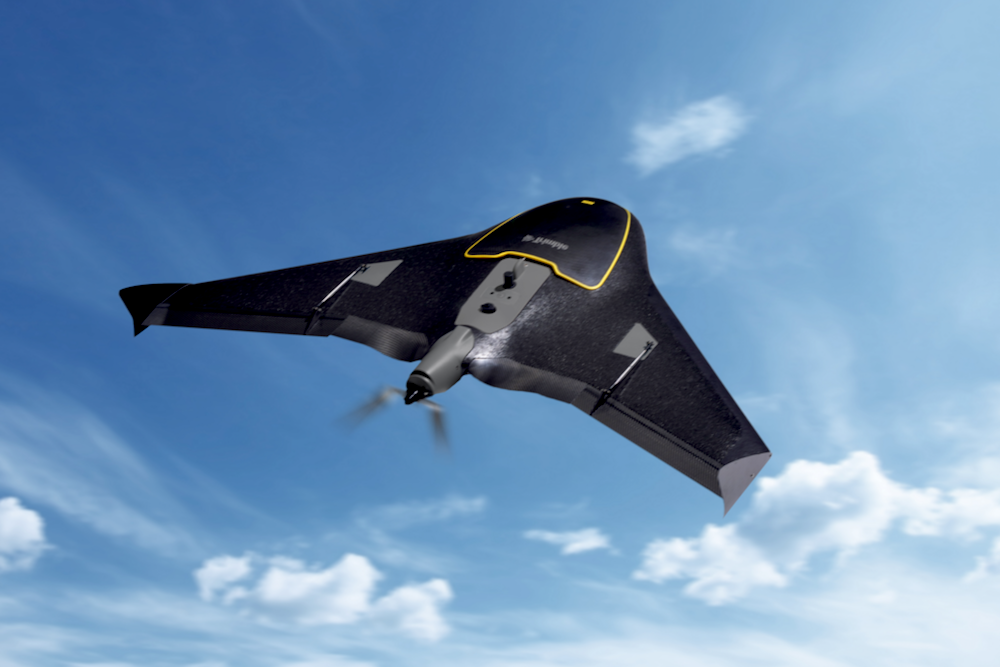
\includegraphics[width=.9\linewidth]{images/fixed-wings-drone.png}
  \caption{Fixed-wing drone}
  \label{fig:uav-fixed-wing}
\end{subfigure}%
\begin{subfigure}{.5\textwidth}
  \centering
  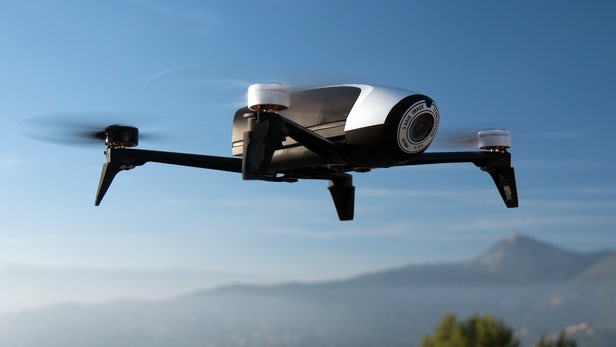
\includegraphics[width=.9\linewidth]{images/quadrotor.jpg}
  \caption{Multi-rotor drone}
  \label{fig:uav-rotor}
\end{subfigure}
\caption{Different types of drones exist. The most common configurations are the fixed-wing and the multi-rotor.}
\label{fig:uav-types}
\end{figure}

\glspl{UAV} are classified depending on a wide range of characteristics: size, range, aerial platform, degree of autonomy, engine type and fuel source. All these features are analysed in this section. \\
The first distinction that can be made is based on the type of aerial platform that is used to keep \glspl{UAV} up in the air. Drones available today belongs to one of two main categories: fixed-wing drones and multi-rotor drones. Fixed-wing drones are equipped with fixed, static wings and they use a forward propulsion to move. The way in which they behave is similar to a traditional airplane. Multi-rotor drones, on the other hand, are more similar to helicopters, since they use one or more rotary wings to generate lift. The most common multi-rotor drones use four rotors and are therefore called quadrotors. Depending on the application, one or the other configuration may be more suitable: fixed-wing drones are typically faster than multi-rotors, but they require more space to take off and they can not hover in a fixed position. Multi-rotor drones can overcome these limitations, but are much slower than fixed-wing models.
\glspl{UAV} can be further divided depending on their size and weight. This characteristic reflects the ability of the drone to carry payloads, with bigger drones being able to carry heavy payloads and small drones only able to carry lightweight payloads. Very small \glspl{UAV} have dimensions of 30-50 cm and are usually multi-rotors. Small \glspl{UAV} are slightly larger (up to 1-2 meters along one dimension) and are usually fixed-wing. The same applies to medium and large \glspl{UAV} with the only difference that they can be as big or bigger than a light aircraft. They can carry very heavy payloads (approximately 200 kg) and are generally only used for military applications. 
\glspl{UAV} engines can be powered using many different fuel sources: traditional aircraft fuel (kerosene or gasoline), fuel cells, batteries and solar cells. With the exception of few models, the vast majority of drones are powered either by aircraft fuel or batteries. Drones using aircraft fuel as their power source are able to fly for longer times, but due to the weight of the fuel and the size of the engine, they have bigger dimensions. The most common engines, in order of stability level they can provide, are the four-cycle/two-cycle internal combustion engine, the rotary engine and the gas turbines. Battery-powered drones, equipped with a simple electric motor, are cheap and lightweight, but their flight autonomy is limited to only a few minutes, thus drastically restricting their application in many context.

\subsection{UAV system}

\begin{figure}[h]
    \centering
    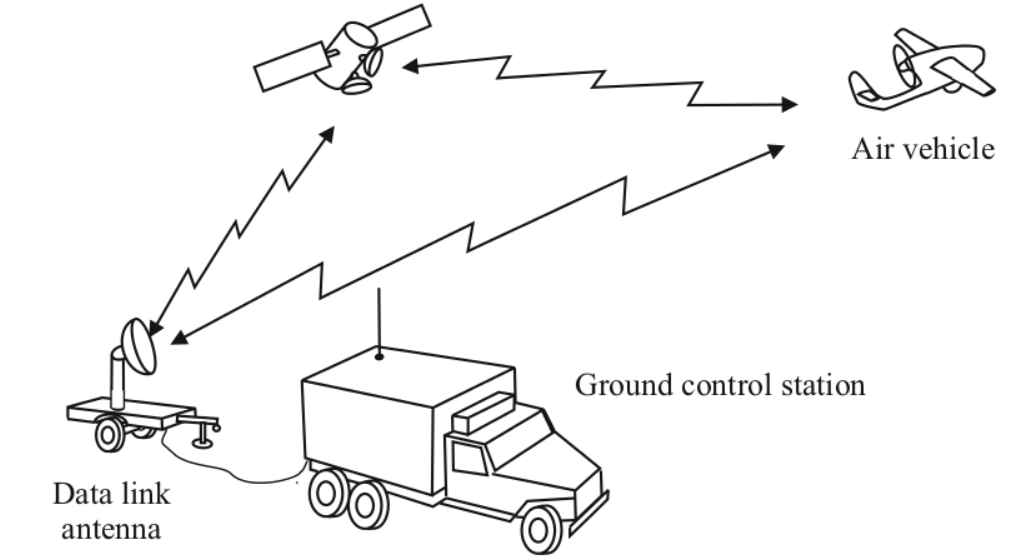
\includegraphics[width=0.9\textwidth]{images/uav-system.png}
    \caption{A general UAV system \ref{undefined}}
    \label{fig:uav-system}
\end{figure}

The operation of one or more \glspl{UAV} requires the deployment of a suitable infrastructure, that is necessary to manage and control all the aspects of the mission. A typical \gls{UAV} system is at least composed by the following elements:

\begin{itemize}
	\item \textbf{Air vehicles:} they are the core part of the system. In order to fly with a high degree of autonomy, air vehicles need to be equipped with some sort of controller that regulate, for example, the altitude and the airspeed. This control is usually achieved by using a feedback or closed-loop controller in conjunction with a set of sensors that typically include an altimeter, a speed meter and some sort of positioning device (a GPS for example). The measurements of the sensors are used by the controller to compute the right actuation to adjust the roll, pitch and/or yaw of the vehicle. Typically the control is limited to one axis (roll) or two axis (roll + pitch) to limit the controller complexity. Almost all \glspl{UAV} are nowadays equipped with a GPS, that can be used to complement the measurements of the other sensors and for accurate path planning;
	
	\item \textbf{Payload:} drones' main mission is to carry a payload. Typical payloads include HD cameras, communication gateways, infrared sensors and thermal sensors. The payload greatly influence the characteristics of the drone that carries it. For example, a heavy payload may require a bigger and more powerful drone;
	
	\item \textbf{\gls{GCS}:} it is usually a vehicle that can transport the drones to the place where they need to operate. The \gls{GCS} is also equipped with all the necessary instruments to process and display the data received from the drones payloads. If the \gls{UAV} system is small, the \gls{GCS} can be reduced to the size of a backpack that can be carried around by the drones operator. A \gls{GCS} can also be located at a fixed position, for example in a building;
	
	\item \textbf{Data link antennas:} antennas are used to establish a two way communication with the air vehicles. The channel is typically split in two sub channels: a low rate channel for transmitting control commands and receiving feedback from the \glspl{UAV} and a high rate channel for receiving sensors data (e.g. the video stream). \gls{LOS} is usually required for the communication to happen;
	
	\item \textbf{\gls{GSE}:} this unit is used to maintain the \glspl{UAV} and may contain spare parts and additional fuel or batteries to extend the \glspl{UAV} on-air time. The \gls{GSE} unit is optional, but its use is generally required, especially in systems with many drones and for missions that require extended operation times.
	
\end{itemize}

%Exclusive prerogative of the military for many years, \glspl{UAV} and drones are now commercially available and their relatively low price makes them appealing for a wide variety of scenarios and applications. The price range can vary between 20\$-300\$ for small battery-powered \gls{RF} drones such as the Parrot Bebop 2, to more than 3000\$ for professional drones with advanced control systems and sensors such as the DJI Spreading Wings S1000. In the consumer market segment, drones are mainly used for taking aerial pictures and videos, while in the commercial segment the range of applications is more diverse: mapping of geographical areas, product delivery and logistic, data collection, crop monitoring and surveillance. Drones are increasingly being used also in civil applications such as crime prevention, weather and meteorology, search and rescue operations, border and maritime patrol and forest fire monitoring. Using \glspl{UAV} provide many advantages compared to ground-based solutions, such as movement in an obstacle-free environment, better overview of the monitored area, presence of \gls{LOS} between the drone and the targets and faster data acquisition over large areas. On the other side, \glspl{UAV} are still limited in terms of flying range, degree of autonomy and flying time. To overcome such issues, \glspl{UAV} swarms are increasingly being considered as a possible solution and many efforts are being directed in the development of suitable communication protocols and swarm mobility models.  
